\documentclass[11pt,a4paper]{article}
\usepackage[utf8]{inputenc}
\usepackage[T1]{fontenc}
\usepackage{amsmath,amssymb,amsfonts}
\usepackage{graphicx}
\usepackage{hyperref}
\usepackage{algorithm}
\usepackage{algorithmic}
\usepackage{cite}
\usepackage{url}
\usepackage{booktabs}
\usepackage{enumitem}
\usepackage{authblk}
\usepackage{tikz}
\usetikzlibrary{arrows.meta,positioning,shapes.geometric,fit}
\usepackage{listings}
\usepackage{xcolor}
\usepackage{multirow}

\definecolor{zoogreen}{RGB}{30,140,60}
\hypersetup{colorlinks=true,linkcolor=zoogreen,citecolor=zoogreen,urlcolor=zoogreen}

\title{\textbf{Zoo EVM: A Post-Quantum Safe Layer 2 Blockchain\\with AI-Native Precompiles on the Lux Network}}

\author[1]{Antje Worring, Zach Kelling\thanks{zach@zoo.ngo}}
\affil[1]{\textit{Zoo Labs Foundation \quad Hanzo Industries \quad Lux Industries}, \texttt{research@zoo.ngo}}

\date{October 2024}

\begin{document}

\zoocoverpage

\begin{abstract}
We present \textbf{Zoo EVM}, a Layer 2 blockchain designed for decentralized artificial intelligence research and decentralized science (DeSci). Operating as a sovereign subnet on the Lux Network, Zoo EVM features 20 precompiles including NIST PQC standards (ML-DSA, SLH-DSA, ML-KEM), threshold signatures (FROST, CGGMP21), privacy primitives (FHE, zero-knowledge proofs, ring signatures), and a novel AI Mining precompile for proof-of-useful-computation consensus. Zoo Labs Foundation, established in 2021 as one of the earliest agentic AI platforms---predating the mainstream adoption of agent frameworks by over two years---brings deep experience in frontier LLM development and decentralized compute to the blockchain layer. This paper describes the architecture, precompile suite, deployment model, and quantum security properties of Zoo EVM, and positions it within the broader Zoo ecosystem of decentralized AI governance via ZIPs (Zoo Improvement Proposals).
\end{abstract}

\section{Introduction}

The convergence of artificial intelligence and blockchain technology demands infrastructure that is simultaneously compute-efficient, cryptographically rigorous, and governance-aware. Centralized AI platforms concentrate model control, training data, and inference revenue in corporate hands. Decentralized alternatives have struggled with the computational intensity of AI workloads and the lack of native cryptographic primitives for model verification, privacy-preserving inference, and threshold custody.

Zoo Labs Foundation was established in 2021 as a 501(c)(3) non-profit research network, pioneering agentic AI systems and frontier language models before ``agentic AI'' entered the mainstream vocabulary. Zoo's early work on autonomous agent coordination, multimodal reasoning, and decentralized training (including the Hamiltonian LLM framework and Training-Free GRPO) demonstrated that meaningful AI research could be conducted outside centralized labs. Zoo EVM extends this mission to the blockchain layer, providing native infrastructure for:

\begin{itemize}[nosep]
  \item \textbf{Post-quantum cryptography}: NIST PQC standards at precompile speed
  \item \textbf{AI Mining}: Proof-of-useful-computation where validators contribute inference/training
  \item \textbf{Privacy-preserving ML}: Fully homomorphic encryption and zero-knowledge proofs for model verification without data exposure
  \item \textbf{Threshold governance}: FROST/CGGMP21 for DAO treasury management
  \item \textbf{DeSci primitives}: On-chain graph operations, experience ledgers, citizen science coordination
\end{itemize}

\section{Architecture}

\subsection{Network Topology}

Zoo EVM operates as an L2 subnet on the Lux Network. The Lux L1 provides validator management (P-Chain), asset transfers (X-Chain), and a general-purpose EVM (C-Chain). Zoo adds a specialized execution environment with 20 precompiles optimized for AI and DeSci workloads.

\begin{center}
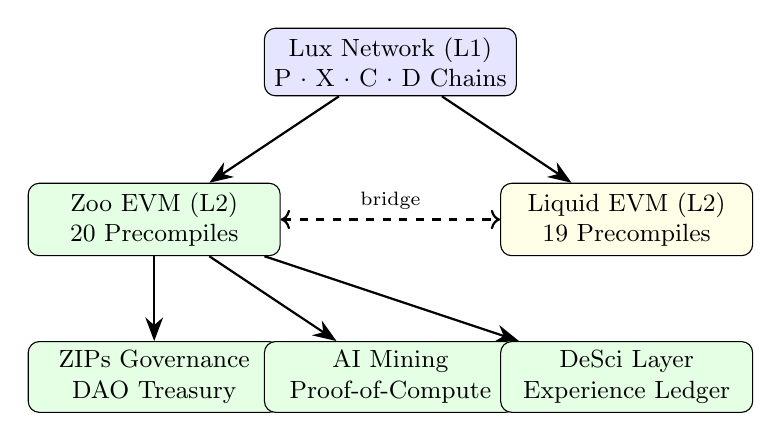
\begin{tikzpicture}[
  box/.style={draw, rounded corners, minimum width=3.2cm, minimum height=0.8cm, align=center, font=\small},
  arrow/.style={-{Stealth[length=3mm]}, thick}
]
  \node[box, fill=blue!10] (lux) at (0,4) {Lux Network (L1)\\P $\cdot$ X $\cdot$ C $\cdot$ D Chains};
  \node[box, fill=green!10] (zoo) at (-3,2) {Zoo EVM (L2)\\20 Precompiles};
  \node[box, fill=yellow!10] (liq) at (3,2) {Liquid EVM (L2)\\19 Precompiles};
  \node[box, fill=green!10] (gov) at (-3,0) {ZIPs Governance\\DAO Treasury};
  \node[box, fill=green!10] (ai) at (0,0) {AI Mining\\Proof-of-Compute};
  \node[box, fill=green!10] (sci) at (3,0) {DeSci Layer\\Experience Ledger};

  \draw[arrow] (lux) -- (zoo);
  \draw[arrow] (lux) -- (liq);
  \draw[arrow] (zoo) -- (gov);
  \draw[arrow] (zoo) -- (ai);
  \draw[arrow] (zoo) -- (sci);
  \draw[<->, dashed, thick] (zoo) -- (liq) node[midway,above,font=\scriptsize] {bridge};
\end{tikzpicture}
\end{center}

\subsection{Chain Parameters}

\begin{table}[h]
\centering
\begin{tabular}{lrrr}
\toprule
\textbf{Parameter} & \textbf{Devnet} & \textbf{Testnet} & \textbf{Mainnet} \\
\midrule
EVM Chain ID & 200202 & 200201 & 200200 \\
Lux Network ID & 3 & 2 & 1 \\
Validators & 5 & 5 & 5 \\
Native Token & ZOO & ZOO & ZOO \\
Total Supply & \multicolumn{3}{c}{1,000,000,000 (1B)} \\
Decimals & \multicolumn{3}{c}{18} \\
Block Gas Limit & \multicolumn{3}{c}{15,000,000} \\
Target Block Rate & \multicolumn{3}{c}{2 seconds} \\
\bottomrule
\end{tabular}
\caption{Zoo EVM chain parameters.}
\end{table}

\subsection{Single-Binary Node Design}

The \texttt{zoo-evm} binary implements a self-installing plugin architecture:

\begin{algorithm}
\caption{Zoo EVM Self-Installing Plugin}
\begin{algorithmic}[1]
\IF{environment variable \texttt{LUX\_VM\_TRANSPORT} is set}
  \STATE Enter EVM plugin mode (subprocess of Lux node)
  \STATE Version: \texttt{Zoo-EVM/\{version\} [node=\{luxd\}, rpcchainvm=\{protocol\}]}
  \STATE Call \texttt{runner.Run(versionStr)}
\ELSE
  \STATE Parse CLI flags via \texttt{config.BuildFlagSet()}
  \STATE Load node configuration
  \STATE Install self as plugin: \texttt{symlink(self, pluginDir/\{EVM\_ID\})}
  \STATE Create Lux node: \texttt{app.New(nodeConfig)}
  \STATE Block: \texttt{app.Run(nodeApp)}
\ENDIF
\end{algorithmic}
\end{algorithm}

This design means one compiled binary serves as both the Lux node process and the EVM plugin subprocess. The node spawns itself as a child process via the plugin symlink, detecting the mode from the \texttt{LUX\_VM\_TRANSPORT} environment variable.

\section{Precompile Architecture}

Zoo EVM activates 20 precompiles at genesis. These execute at native speed within the EVM, avoiding the 100--1000x overhead of implementing equivalent operations in Solidity bytecode.

\begin{table}[h]
\centering
\small
\begin{tabular}{llll}
\toprule
\textbf{Category} & \textbf{Precompile} & \textbf{Address} & \textbf{Standard} \\
\midrule
\multirow{5}{*}{Post-Quantum} & ML-DSA & \texttt{0x0200...06} & FIPS 204 \\
 & SLH-DSA & \texttt{0x0600...01} & FIPS 205 \\
 & ML-KEM & \texttt{0x0200...07} & FIPS 203 \\
 & PQCrypto & \texttt{0x...9003} & Composite \\
 & Blake3 & \texttt{0x0500...04} & BLAKE3 \\
\midrule
\multirow{3}{*}{Threshold Sig} & FROST & \texttt{0x0800...02} & RFC 9591 \\
 & CGGMP21 & \texttt{0x0800...03} & CGGMP21 \\
 & Corona & \texttt{0x0200...0B} & Ring-CT \\
\midrule
\multirow{3}{*}{Curves} & Ed25519 & \texttt{native} & RFC 8032 \\
 & secp256r1 & \texttt{native} & NIST P-256 \\
 & SR25519 & \texttt{native} & Ristretto \\
\midrule
\multirow{4}{*}{Privacy} & FHE & \texttt{0x0700...00} & CKKS/BGV \\
 & ZK & \texttt{0x0900...00} & Groth16 \\
 & HPKE & \texttt{0x...9200} & RFC 9180 \\
 & ECIES & \texttt{0x...9201} & IEEE 1363a \\
\midrule
Privacy & Ring & \texttt{0x...9202} & Borromean \\
\midrule
\multirow{2}{*}{DeFi} & DEX Pool & \texttt{0x...9010} & Uniswap v4 \\
 & Router & \texttt{0x...9012} & Swap Router \\
\midrule
\textbf{AI} & \textbf{AI Mining} & \texttt{0x0300...00} & \textbf{PoUC} \\
\midrule
Compute & Graph & \texttt{0x0500...10} & On-chain GNN \\
\bottomrule
\end{tabular}
\caption{Zoo EVM precompile suite. AI Mining (bold) is unique to Zoo---not present on Liquid EVM.}
\end{table}

\subsection{Post-Quantum Cryptography}

Zoo EVM implements all three NIST PQC standards finalized in 2024:

\textbf{ML-DSA} (FIPS 204): Module-Lattice Digital Signature Algorithm. Provides quantum-resistant digital signatures based on the hardness of Module Learning With Errors (MLWE). Zoo uses ML-DSA-65 (Level 3, 3.3 KB signatures) for validator attestations and governance votes.

\textbf{SLH-DSA} (FIPS 205): Stateless Hash-Based Digital Signature Algorithm. Provides signatures with minimal cryptographic assumptions (only hash function security). Larger signatures (17 KB for SLH-DSA-SHAKE-256f) but maximum conservative security. Used for long-term key certification.

\textbf{ML-KEM} (FIPS 203): Module-Lattice Key Encapsulation Mechanism. Provides quantum-resistant key exchange. Used in MPC keygen ceremonies and secure channel establishment between validators.

\subsection{AI Mining Precompile}

The AI Mining precompile at \texttt{0x0300...00} enables proof-of-useful-computation (PoUC):

\begin{enumerate}[nosep]
  \item \textbf{Task submission}: Research tasks (inference, training batches, evaluation) are posted on-chain with compute requirements and reward allocation.
  \item \textbf{Compute commitment}: Validators commit to executing tasks, staking ZOO as collateral.
  \item \textbf{Result verification}: Completed results are submitted with cryptographic proofs. For deterministic tasks (inference), bit-exact reproducibility is verified. For stochastic tasks (training), statistical validation against held-out test sets is used.
  \item \textbf{Reward distribution}: Verified compute earns ZOO rewards plus governance rights (ZIPs voting weight).
\end{enumerate}

This mechanism transforms idle validator compute into productive AI research capacity, aligning economic incentives with scientific output.

\subsection{Privacy Precompiles for ML}

Two precompiles enable privacy-preserving machine learning:

\textbf{FHE} (Fully Homomorphic Encryption): The CKKS/BGV precompile at \texttt{0x0700...00} enables computation on encrypted data. Applications include private model inference (user data never decrypted on-chain) and encrypted model parameter aggregation in federated learning.

\textbf{ZK} (Zero-Knowledge Proofs): The Groth16 precompile at \texttt{0x0900...00} enables succinct verification of computation. Applications include proving model accuracy without revealing model weights, verifying training data provenance, and privacy-preserving credential verification for DeSci access control.

\section{Deployment Architecture}

\subsection{Kubernetes Infrastructure}

Zoo EVM runs on a dedicated DigitalOcean Kubernetes cluster:

\begin{table}[h]
\centering
\begin{tabular}{ll}
\toprule
\textbf{Property} & \textbf{Value} \\
\midrule
Cluster & \texttt{do-sfo3-zoo-k8s} (DigitalOcean SFO3) \\
Nodes & 5 $\times$ s-4vcpu-8gb-amd \\
Kubernetes & v1.35.1 \\
Namespaces & zoo-system, zoo-devnet, zoo-testnet, zoo-mainnet \\
Image Registry & DOCR (\texttt{registry.digitalocean.com/hanzo/}) \\
\bottomrule
\end{tabular}
\caption{Zoo K8s cluster configuration.}
\end{table}

\subsection{Zoo Operator}

The Zoo Operator is a Rust-based Kubernetes operator managing four Custom Resource Definitions:

\begin{description}[nosep]
  \item[ZooNetwork] (\texttt{zoo.network/v1alpha1}): Primary CRD for deploying validator node clusters. Creates StatefulSets, headless Services, and manages rolling upgrades.
  \item[ZooChain] Tracks EVM chain deployments (chain ID, blockchain ID, VM ID).
  \item[ZooExplorer] Manages Blockscout instances for each chain.
  \item[ZooGateway] Manages RPC gateway/ingress for Zoo EVM endpoints.
\end{description}

The operator implements leader election via Kubernetes Lease objects and exposes Prometheus metrics for reconciliation monitoring.

\section{Comparison with Liquid EVM}

Zoo EVM and Liquid EVM share the Lux L1 base layer and 19 common precompiles but serve distinct purposes:

\begin{table}[h]
\centering
\small
\begin{tabular}{lll}
\toprule
\textbf{Property} & \textbf{Zoo EVM} & \textbf{Liquid EVM} \\
\midrule
Purpose & DeSci / DeAI research & Securities settlement \\
Token & ZOO (1B supply) & LQDTY (10B supply) \\
Chain IDs & 200200/01/02 & 8675309/10/11 \\
Precompiles & 20 (incl. AI Mining) & 19 (no AI Mining) \\
Governance & ZIPs (zoo.ngo) & Corporate (ATS/BD/TA) \\
Custody & 2-of-3 MPC (treasury) & 2-of-3 MPC (per-user) \\
Operator CRDs & 4 (chain-focused) & 18 (chain + platform) \\
Cluster & DOKS (zoo-k8s) & GKE (zoo-chains) \\
Dollar token & None & USDL \\
Established & 2021 & 2022 \\
\bottomrule
\end{tabular}
\caption{Zoo EVM vs Liquid EVM architectural comparison.}
\end{table}

The two chains can interoperate via the Lux C-Chain bridge, enabling DeSci assets to be traded on the Lux exchange and USDL to fund Zoo research bounties.

\section{ZIPs Governance Integration}

Zoo Improvement Proposals (ZIPs) at \texttt{zips.zoo.ngo} provide on-chain governance for the Zoo ecosystem. The ZooNetwork CRD supports DAO-controlled parameter updates:

\begin{itemize}[nosep]
  \item Precompile activation/deactivation via governance vote
  \item AI Mining reward rate adjustment
  \item Validator set changes (proof-of-stake + proof-of-compute)
  \item Research fund allocation from treasury
\end{itemize}

100 ZIPs have been proposed to date, covering topics from training infrastructure (ZIP-001) to semantic reranking (ZIP-002) to federated learning protocols.

\section{Security Considerations}

\subsection{Quantum Threat Timeline}

Current estimates place cryptographically relevant quantum computers (CRQC) at 2030--2035. Zoo EVM's hybrid approach provides immediate classical security (ECDSA) with quantum-resistant backup (ML-DSA/SLH-DSA). Key migration procedures are defined: if ECDSA is compromised, ML-DSA attestations enable trustworthy key rotation.

\subsection{Threshold Custody}

Zoo treasury funds are managed via 2-of-3 MPC (CGGMP21 for ECDSA, FROST for EdDSA). This prevents single-point-of-compromise scenarios. Shamir backup enables recovery if one key share is lost.

\subsection{AI Mining Security}

The AI Mining precompile mitigates compute fraud through:
\begin{itemize}[nosep]
  \item Deterministic task replay for verification
  \item Statistical validation for stochastic tasks
  \item Slashing conditions for fraudulent results
  \item Rate limiting to prevent compute exhaustion attacks
\end{itemize}

\section{Conclusion}

Zoo EVM provides the first post-quantum safe, AI-native Layer 2 blockchain for decentralized science and AI research. By combining NIST PQC standards, threshold signatures, privacy-preserving computation, and proof-of-useful-computation mining, Zoo creates infrastructure where scientific progress and economic incentives are cryptographically aligned. The 20-precompile suite, Kubernetes-native operator, and three-network deployment provide a production-ready foundation for the next generation of decentralized AI.

Building on Zoo Labs Foundation's 2021 origins as a pioneer in agentic AI---years before the term became mainstream---Zoo EVM extends the principle that AI infrastructure should be community-owned, scientifically rigorous, and quantum-safe from day one.

\begin{thebibliography}{99}
\bibitem{lux-consensus} Kelling, Z. ``Lux Consensus: Multi-Engine Blockchain Consensus.'' Lux Industries, 2025.
\bibitem{lux-pq} Kelling, Z. ``EthFalcon: Post-Quantum Cryptography for EVM Chains.'' Lux Industries, 2025.
\bibitem{lux-precompiles} Kelling, Z. ``Lux EVM Precompiles: Native Cryptographic Primitives.'' Lux Industries, 2025.
\bibitem{liquid-evm} Kelling, Z. ``Liquid EVM: On-Chain Securities Settlement with Post-Quantum MPC Custody.'' Lux Exchange, 2026.
\bibitem{zoo-network} Kelling, Z. ``Zoo Network: Decentralized AI Training and Inference Layer.'' Zoo Labs Foundation, 2025.
\bibitem{zoo-experience} Kelling, Z. ``The Experience Ledger: Content-Addressable Semantic Optimization Knowledge.'' Zoo Labs Foundation, 2025.
\bibitem{cggmp21} Canetti, R., et al. ``UC Non-Interactive, Proactive, Threshold ECDSA.'' ACM CCS 2020.
\bibitem{frost} Komlo, C., Goldberg, I. ``FROST: Flexible Round-Optimized Schnorr Threshold Signatures.'' SAC 2020.
\bibitem{fips204} NIST. ``FIPS 204: Module-Lattice-Based Digital Signature Standard.'' 2024.
\bibitem{fips205} NIST. ``FIPS 205: Stateless Hash-Based Digital Signature Standard.'' 2024.
\bibitem{fips203} NIST. ``FIPS 203: Module-Lattice-Based Key-Encapsulation Mechanism Standard.'' 2024.
\end{thebibliography}

\end{document}
